\begin{frame}{root servers (1)}
(from IANA's website)
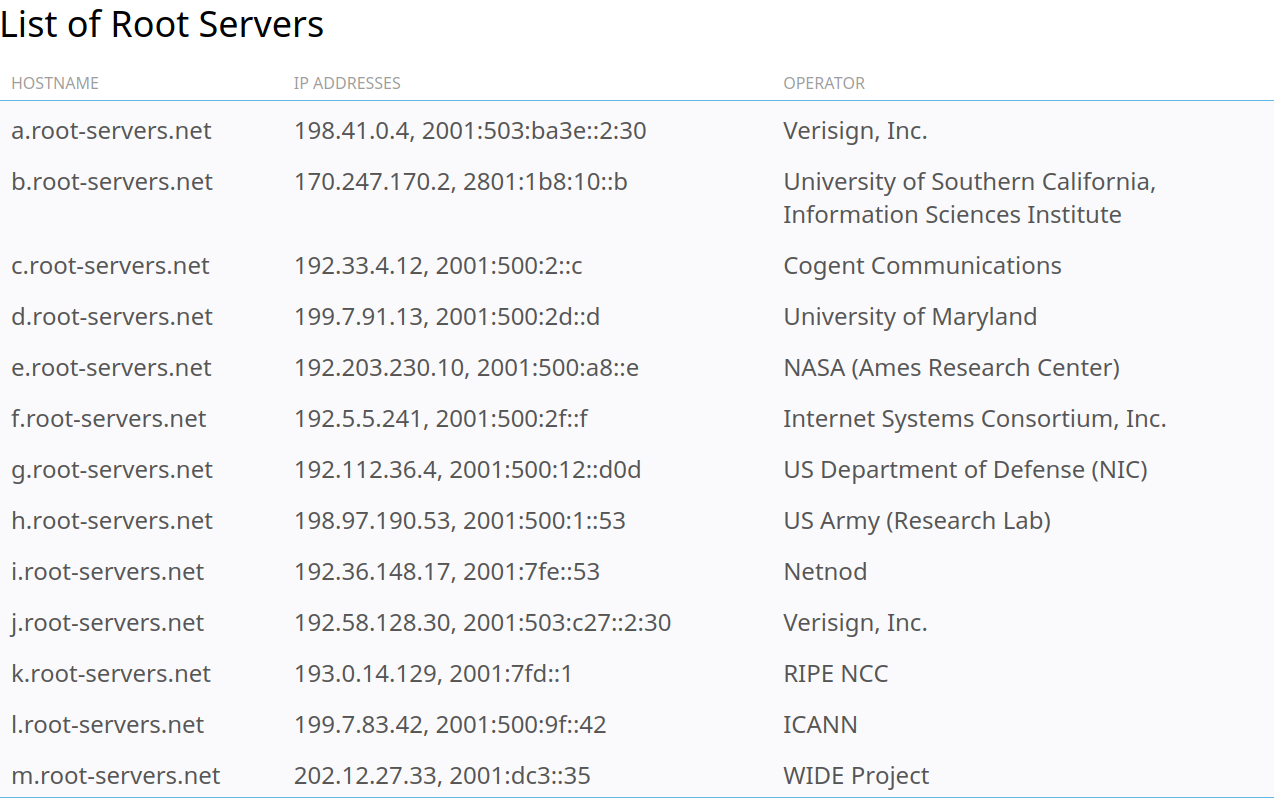
\includegraphics[height=0.8\textheight]{iana-root-server-list}
\end{frame}

\begin{frame}{root servers (2)}
(from root-servers.org)
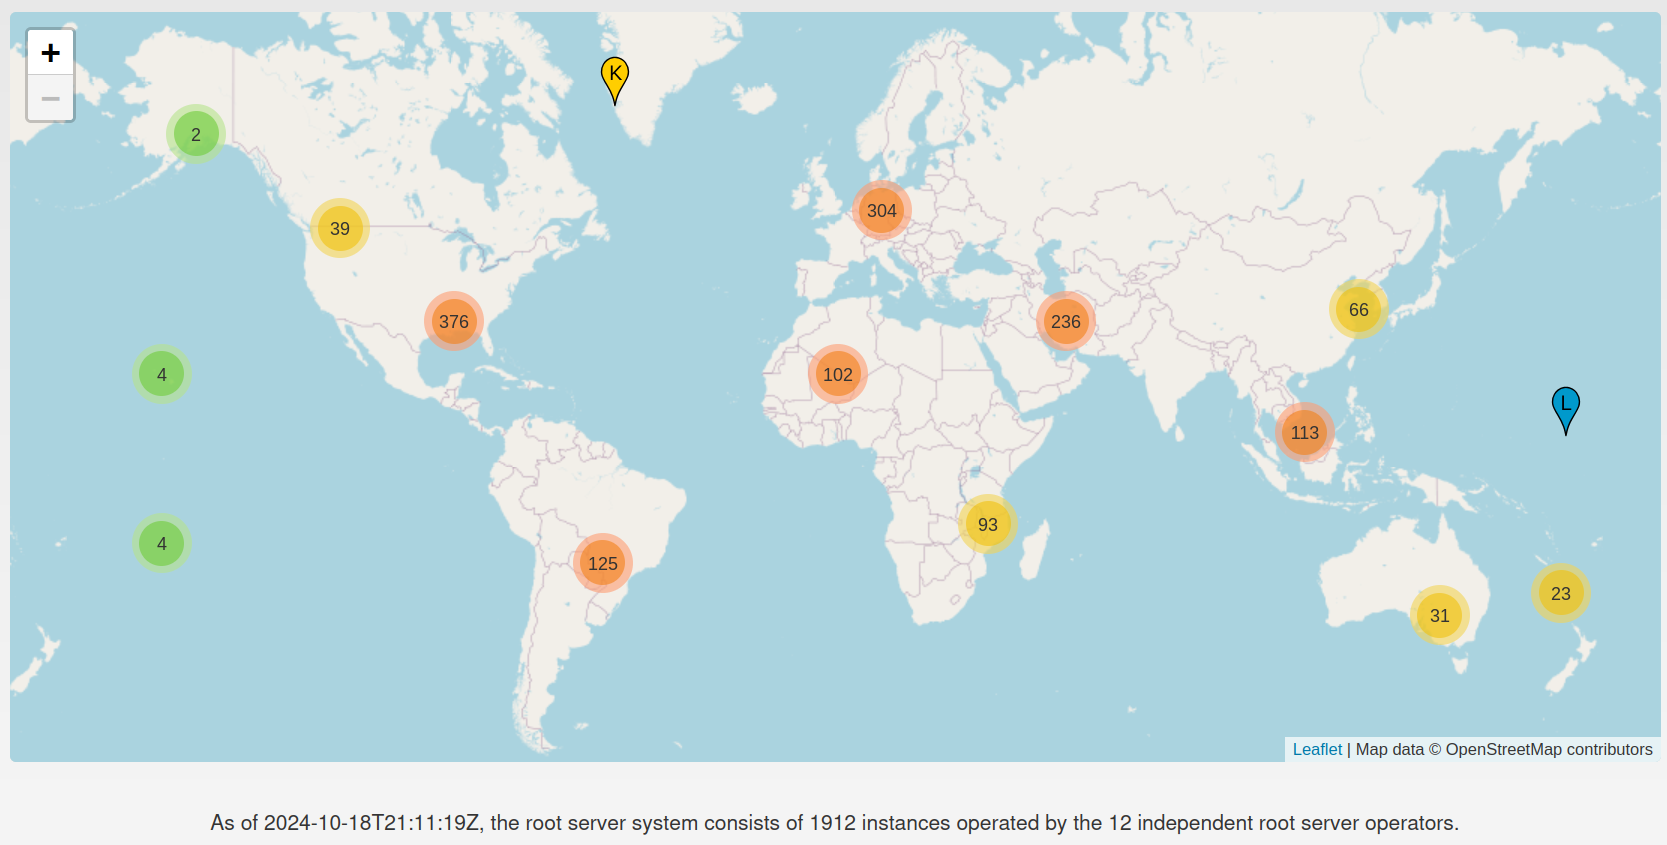
\includegraphics[width=0.9\textwidth]{root-servers-map}
\end{frame}

\begin{frame}{anycast root servers}
    \begin{itemize}
    \item many root servers have multiple separate sites
    \item \ldots but one IPv4/IPv6 address
    \vspace{.5cm}
    \item which one you get = which one routed to
    \item multiple sites with BGP announcements for IP
        \begin{itemize}
        \item often with care taken to limit how far route goes
        \end{itemize}
    \item idea called `anycast'
        \begin{itemize}
        \item get to `any' of several servers
        \end{itemize}
    \item also used for some public recursive DNS servers
        \begin{itemize}
        \item 1.1.1.1 (CloudFlare), 8.8.8.8 (Google), 208.67.222.222 (Cisco), \ldots
        \end{itemize}
    \end{itemize}
\end{frame}
